% Created 2019-11-10 dom 10:45
% Intended LaTeX compiler: pdflatex
\documentclass[11pt]{article}
\usepackage[utf8]{inputenc}
\usepackage[T1]{fontenc}
\usepackage{graphicx}
\usepackage{grffile}
\usepackage{longtable}
\usepackage{wrapfig}
\usepackage{rotating}
\usepackage[normalem]{ulem}
\usepackage{amsmath}
\usepackage{textcomp}
\usepackage{amssymb}
\usepackage{capt-of}
\usepackage{hyperref}
\usepackage[newfloat]{minted}
\hypersetup{colorlinks=true,linkcolor=black}
\usepackage{mathpazo}    %fuente palatino
\usepackage{charter}      %fuente charter
\linespread{1.05}         %separa un poco las líneas para que no quede apelotonado
\author{Angel Berlanas Vicente}
\date{\today}
\title{La Memoria RAM\\\medskip
\large Montaje Y Mantenimiento}
\hypersetup{
 pdfauthor={Angel Berlanas Vicente},
 pdftitle={La Memoria RAM},
 pdfkeywords={},
 pdfsubject={},
 pdfcreator={Emacs 25.2.2 (Org mode 9.2.5)}, 
 pdflang={Spanish}}
\begin{document}

\maketitle
\tableofcontents


\section{Glosario}
\label{sec:org99c87e5}

En general, la memoria del sistema se encarga de almacenar los datos, de forma que
esta esté accesible para la CPU. El sistema de memoria de los ordenadores modernos
consta de varias secciones con diferentes tareas:

\begin{itemize}
\item La memoria de trabajo o RAM (Random Access Memory) es la memoria principal
del  ordenador que se puede leer y escribir con rapidez. Es volátil, es
decir, pierde sus  datos al apagar el ordenador. El tamaño de la memoria RAM
en los ordenadores actuales se mide en megabytes o gigabytes.
\item La memoria caché. Es más rápida que la memoria RAM y se usa para acelerar la
transferencia de datos. En ella se almacenan datos de la memoria principal a
los que accederá el microprocesador próximamente. Justo antes de necesitar
esos datos, se seleccionan y se colocan en dicha memoria. Ya vimos los tipos de caché L1, L2 y L3.
\item La memoria CMOS, que almacena datos de configuración física del equipo. Al ejecutar el programa Setup se pueden cambiar los datos almacenados allí.
\item La ROM o memoria de solo lectura (Read Only Memory). Aunque es solo de
lectura, sí se puede modificar una o más veces, dependiendo del tipo de
ROM. La BIOS de los ordenadores actuales está grabada en una ROM (EEPROM),
más conocida como Flash-ROM, que nos permitirá actualizarla.
\item La memoria gráfica o de vídeo. Dedicada a satisfacer las necesidades de la
tarjeta gráfica. Muchas tarjetas gráficas la llevan integrada, pero otras de
gama baja emplean parte de la memoria RAM para aplicaciones tales como los juegos 3D.
\end{itemize}

Algunos parámetros que hay que tener en cuenta en la memoria son:

\begin{itemize}
\item La \textbf{velocidad}. Se mide en megahercios (MHz). Por ejemplo, si la velocidad de
una memoria es de 800 MHz, significa que con ella se pueden realizar 800
millones de operaciones (lecturas y escrituras) en un segundo.
\item El \textbf{ancho de band} a o tasa de transferencia de datos. Es la máxima cantidad de
memoria que puede transferir por segundo, se expresa en megabytes por segundo
(MB/s) o en gigabytes por segundo (GB/s).
\item \emph{Dual/triple channel}. Permite a la CPU trabajar con dos/tres canales
independientes y simultáneos para acceder a los datos. De esta manera se
multiplica el ancho de banda. Para ello, es imprescindible rellenar los
bancos de memoria con dos o tres módulos de idénticas características.
\item \textbf{Tiempo de acceso}. Es el tiempo que tarda la CPU en acceder a la memoria. Se
mide en nanosegundos (un nanosegundo = 10–9 segundos).
\item \textbf{Latencia}. Es el retardo producido al acceder a los distintos componentes de la memoria RAM.
\item \textbf{Latencias CAS o CL}. Indica el tiempo (en número de ciclos de reloj) que
transcurre desde que el controlador de memoria envía una petición para leer
una posición de  memoria hasta que los datos son enviados a los pines de
salida del módulo. Cuanto menor sea, más rápida será la memoria. A veces se
abrevia como CL (Cas Latency) o CAS.
\item \textbf{ECC} (Error Checking and Correction). Todas las memorias RAM experimentan
errores, debido a factores tales como fluctuaciones de energía,
interferencias, componentes defectuosos, etc. Las memorias ECC son capaces de
detectar y corregir algunos de estos errores.
\end{itemize}


\section{Tipos de RAM}
\label{sec:org6667c5e}

Cuando ejecutamos un programa en el ordenador se pasa una copia de este desde
el almacenamiento secundario, que normalmente es el disco duro, a la memoria
RAM. Una vez en la memoria, las instrucciones que componen el programa pasan
a la CPU para su ejecución. ¿Por qué se utiliza la memoria RAM? Porque puede transferir datos desde y hacia la CPU mucho más rápido que los dispositivos de almacenamiento secundario. Si no hubiese memoria RAM, todas las instrucciones y los
datos se leerían de la unidad de disco, lo que reduciría la velocidad de
proceso del ordenador.
Los dos tipos básicos de memoria RAM utilizados en un ordenador personal son
la DRAM (memoria RAM dinámica) y la SRAM (memoria RAM estática). Ambas
almacenan datos e instrucciones, pero son bastante diferentes y cada una tiene un
propósito.

\subsection{Descripción de los tipos}
\label{sec:org3baeab9}

\subsubsection{SRAM-RAM}
\label{sec:org9eb7a27}

Esta memoria,al ser estática, mantiene la información siempre que no se interrumpa
la alimentación. Las memorias SRAM ocupan más tamaño, tienen
menos capacidad y son más caras y rápidas que las DRAM. No se
suelen utilizar como memoria principal, sino como memorias cachés
del microprocesador y de la placa base.

\subsubsection{DRAM-RAM}
\label{sec:org6ba5aa8}

Es la memoria principal de los ordenadores personales. Se la llama
dinámica porque su contenido se reescribe continuamente.
Al ser la memoria principal, la DRAM ha tenido que adaptarse
para seguir el ritmo de evolución de los microprocesadores y demás
conjuntos de chips. Veremos a continuación las tecnologías más
comunes.

\subsubsection{SDRAM-DRAM}
\label{sec:org4fe70d2}
Se sincroniza con el reloj del sistema para leer y escribir en   modo ráfaga. 
Puede soportar velocidades de la placa base de 100 MHz y 133 MHz (más
conocidas como PC100/PC133 SDRAM).
La memoria SDRAM tiene un ancho de bus de datos de 64 bits; en
cada hercio (Hz) (o ciclo de reloj) envía 64 bits (8 B). Calculamos los
bytes que se envían por segundo a 100 y 133 MHz, o sea, la tasa
de transferencia:

\begin{itemize}
\item PC100: 8 bytes/Hz × 100 MHz = 800 MB/s.
\item PC133: 8 bytes/Hz × 133 MHz = 1066 MB/s.
\end{itemize}

Normalmente son suministradas en módulos DIMM de \textbf{168} pines con
dos ranuras.

\subsubsection{DDR SDRAM-SDRAM}
\label{sec:org0d8d98a}

Es una memoria de doble tasa de transferencia
de datos que permite la transferencia de datos por dos canales
distintos simultáneamente en un mismo ciclo de reloj. Supone una
mejora con respecto a la SDRAM, ya que consigue duplicar la
velocidad de operación hasta los 200 MHz o 266 MHz. Se la
conoce más como DDR.
Normalmente son suministradas en módulos DIMM con \textbf{184} pines
con una sola ranura.

\subsubsection{DDR2 SDRAM.}
\label{sec:org87f84f2}

Supone una mejora con respecto a la DDR SDRAM,
ya que funciona a más velocidad y necesita menos voltaje, con
lo que se reduce el consumo de energía y la generación de calor.
La tasa de transferencia de datos va de 400 hasta 1 024 MB/s y
permite capacidades de hasta 2 GB (por módulo). La pega es que
las latencias son más altas que en las DDR. Son suministradas en
módulos DIMM con \textbf{240} pines y una sola ranura.

\subsubsection{DDR3 SDRAM.}
\label{sec:orgf989889}

Esta supone una mejora con respecto a la DDR2
SDRAM: mayor tasa de transferencia de datos, menor consumo
debido a su tecnología de fabricación y permite módulos de mayor
capacidad, hasta 8 GB. También tiene sus inconvenientes, las
latencias son más altas que en las DDR2. También son suministradas
en módulos DIMM con \textbf{240} pines.

\subsubsection{DDR4 SDRAM}
\label{sec:org5991cda}

Los módulos de memoria DDR4 SDRAM tienen un total de \textbf{288} pines DIMM. La
velocidad de datos por pin,  va de un mínimo de 1,6 Gb hasta un máximo inicial
de 3,2 Gb/s.
​
Las memorias DDR4 SDRAM tienen un mayor rendimiento y menor consumo que las
memorias DDR predecesoras. Tienen un gran ancho de banda en comparación con sus
versiones anteriores.

\subsubsection{VRAM (Video Random Access Memory).}
\label{sec:orgd5c1e2c}

Es un tipo de memoria RAM
utilizada por la tarjeta gráfi ca para poder manejar la información
visual que le envía la CPU. Este tipo de memoria permite a la CPU
almacenar información en ella mientras se leen los datos que serán
visualizados en el monitor.


\section{Tipos de Módulos de Memoria RAM}
\label{sec:org26d34ea}

\subsection{DIMM}
\label{sec:org009ff35}

Módulo de memoria en línea doble. El formato DIMM es
similar al SIMM, pero físicamente es más grande y tiene 168
contactos. Se distingue por tener una muesca en los dos lados
y otras dos en la fila de contactos. Se monta en los zócalos de
forma distinta a los SIMM. Existen módulos DIMM de 32, 64,
128, 256 y 512 Mb y de 1, 2 o más gigabytes.

\subsection{DIMM DDR}
\label{sec:org39a98b0}

Los módulos DIMM DDR han sustituido a los módulos DIMM
estándar. Estos vienen con 184 contactos. Los módulos de
memoria parecen iguales, pero los DIMM DDR tienen una única
muesca en la fila de contactos.
Los módulos DIMM DDR2 tienen 240 pines y una muesca en
una posición diferente a los DIMM DDR. También las ranuras
donde se insertarán los módulos de memoria son diferentes.
Los módulos DIMM DDR3 tienen el mismo número de pines
que los DIMM DDR2, pero son física y eléctricamente
incompatibles

\subsection{FB-DIMM \emph{(Fully Buffered DIMM)}}
\label{sec:org274db26}

La módulos de memoria FB-DIMM se suelen utilizar en
servidores. Los datos entre el módulo y el controlador de
memoria se transmiten en serie, con lo que el número de líneas
de conexión es inferior; esto proporciona grandes mejoras en
cuanto a la velocidad y a la capacidad de la memoria. Tiene
las desventajas de su elevado coste, el calor generado debido
al aumento de velocidad y el incremento de la latencia. Los
módulos FBDIMM tienen 240 pines, como los DDR2, pero la
posición de sus muescas es distinta.

\subsection{GDDR}
\label{sec:orga6c17ba}

Son chips de memoria insertados en algunas tarjetas gráficas o en placas
base donde la tarjeta gráfica está integrada. Son memorias muy rápidas,
controladas por el procesador de la tarjeta gráfica. También se los conoce
como RAM DDR para gráficos.

\subsection{SO-DIM y Micro-DIMM}
\label{sec:org46df1e0}

Son módulos DIMM de memoria para portátiles; el segundo tiene un formato más pequeño que el primero. Los SO-DIMM para memorias
DDR y DDR2 se diferencian porque tienen la muesca en distinta posición.

\subsection{Módulos buffered y unbuffered}
\label{sec:org13d6d82}

Los módulos \textbf{buffered} o registered tienen registros incorporados (circuitos que aseguran la estabilidad a costa de perder rendimiento) que actúan como almacenamiento
intermedio entre la CPU y la memoria. Este tipo de memoria aumenta la fiabilidad del
sistema, pero también retarda los tiempos de transferencia de datos entre esta y
el sistema. 

Se suelen usar sobre todo en servidores, donde es mucho más importante la
integridad de los datos que la velocidad. Los módulos registered se distinguen de los
unregistered por tener varios chips de pequeño tamaño. Incluyen detección y corrección de errores (ECC).

Los módulos \textbf{unbuffered} o unregistered se comunican directamente con el northbridge
de la placa base. Esto hace que la memoria sea más rápida, aunque menos segura que
la registered.

\begin{center}
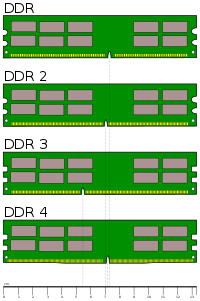
\includegraphics[width=.9\linewidth]{./imgs/DDR.png}
\end{center}

\section{Ejercicios}
\label{sec:org30cc413}

Realizar todos los ejercicios en un fichero \emph{PDF} y copiar el enunciado antes de
contestar.

\subsection{Ejercicio 1}
\label{sec:orgb3ebe03}

¿Qué es la memoria \emph{SWAP}? Explica cómo funciona en GNU/LinuX si estamos usando
una partición y cómo funciona si estamos usando un Fichero.

\subsection{Ejercicio 2}
\label{sec:orge95d683}

En los sistemas Windows, el fichero de SWAP se aloja en \texttt{PAGEFILE.SYS},
describe cómo podríamos cambiarlo.

\subsection{Ejercicio 3}
\label{sec:org0d28695}

Elabora una tabla compartiva de los voltajes a los que funcionan los
diferentes módulos de RAM que hemos visto.

\subsection{Ejercicio 4}
\label{sec:orga6907be}

El comando \texttt{free} nos muestra la cantidad de memoria usada y libre en el
sistema.

Leyendo su página de manual (\texttt{man free}), contesta a las siguientes
preguntas:

\begin{itemize}
\item ¿Cómo obtendríamos el estado de la RAM cada 3 segundos?
\item ¿Y si lo quisiéramos con los totales expresados en \emph{mebibytes}?
\item ¿Qué significa el uso del parámetro \texttt{-h}?
\item ¿Qué hace el argumento \texttt{-{}-si}?¿Porqué es necesario?
\end{itemize}
\end{document}
